\chapter{Fundamental Concepts}
In this chapter I will lay out the fundamental concepts, which are necessary in order to understand the subsequent chapters.
First I will explain Stream Processing in 2.1, afterwards the concept of the MAPE-K Loop will be presented and explained in subchapter 2.1 
followed by a brief explanation of self-adaptive systems to conclude this chapter.

    \section{Stream Processing}
    In this section I will split the concept of Stream Processing into three further components.
    In 2.1.1 I will then define Stream Processing Systems, explain how they work and give examplary fields of application.
    Afterwards in 2.1.2 I will then move onto the topic of Data Stream Management Systems and finally in 2.1.3 I will talk about
    some requirements that SPS should meet.
    
        \subsection{Stream Processing Systems}
        This subsection should explain what stream processing systems are, how they work, what kind of SPS are around
        \textbf{TODO: Wie sieht Data in SPS aus? discuss with DBMS approach, too}
        An SPS takes in one or multiple continuous streams of data, each element of the stream then gets processed by a number of operators and eventually, 
        the SPS puts out a stream of processed data.
    
        In order to increase efficiency, an SPS can, if (computational) resources are available, create replicas of operators to introduce parallelity. 
        Conversely, if there is little input, it may also reduce the amount of replicas in order to save or free up additional resources, as shown in figure 2.1.
        \begin{figure}[h]
        \centering
        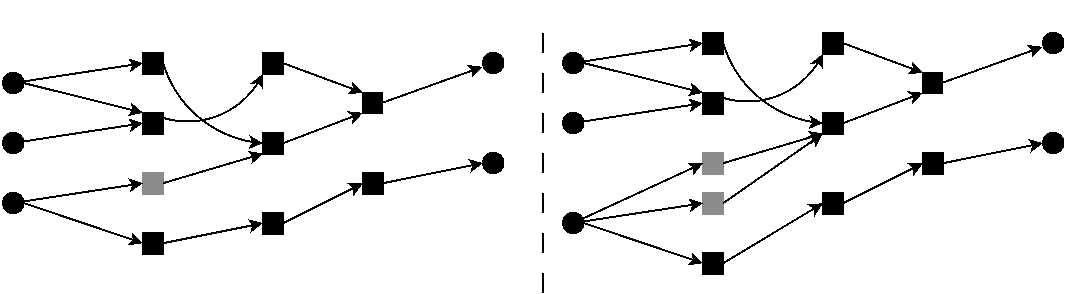
\includegraphics[width=1.0\textwidth]{Bilder/sps_parallel_normal.png}
        \caption{
                Left: An example for an SPS displayed as a directed acyclic graph. 
                Right: Same SPS with introduced parallelity in one operator, marked gray for visibility. 
                Circles are input/outputs, squares are operators, arrows are streams.
                }
        \label{fig:sps_parallel_normal}
        \end{figure}

        \begin{figure}[h]
        \centering
        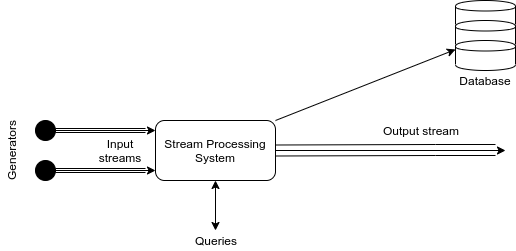
\includegraphics[width=1.0\textwidth]{Bilder/stream-processing-system.png}
        \caption{
                Overview of a basic Stream Processing System
                }
        \label{fig:stream-processing-system}
        \end{figure}
        \subsection{Data Stream Management Systems}
        what are dsms, why dsms as opposed to dbms

        \begin{table}[h]
            \centering
            \label{tab:dbms-dsms}
            \begin{tabular}{|c|c|c|} \hline
                \textbf{Feature} & \textbf{DBMS} & \textbf{DSMS} \\ \hline
                Model & Persistent data & Transient Data \\ \hline
                Table & Set or bag of tuples & Infinite sequence of tuples \\ \hline
                Updates & All & Append only \\ \hline
                Queries & Transient & Persistent \\ \hline
                Query answers & Exact & Often approximate \\ \hline
                Query evaluation & Blocking and non-blocking & Non-blocking \\ \hline
                Operators & Fixed & Adaptive \\ \hline
                Data processing & Synchronous & Asynchronous \\ \hline
                Concurrency overhead  & High & Low \\ \hline
            \end{tabular}
            \captionbelow{Functional comparison of DBMS and DSMS\cite{Panigati2015}} 
        \end{table}

        % Subsection Requirements for Stream Processing Systems
        % Should quickly go over the requirements and explain why they matter to us
        \subsection{Requirements for Stream Processing Systems}
        What are the requirements, why do they matter to us (Elaborate on this)

        Due to the nature of the fields in which SPS are used, there are important requirements that SPS should meet in order to be viable, 
        which Stonebraker et al. point out in \cite{Stonebraker:2005:RRS:1107499.1107504}, of which the ones most important to us can be summarized as the following:
        
        % Enumeration of requirements for SPS + explanations why they matter to us
        \begin{enumerate}
            \item \textbf{Keep the Data Moving:} 
                In order to minimize latency, data must not be stored, as these are costly operations.
            \item \textbf{Handle Stream Imperfections:} 
                Expecting only perfect data is utopian, so one must prepare the system with built-in mechanisms for data that might be missing or out-of-order.
            \item \textbf{Integrate Stored and Streaming Data:} 
                For an SPS to be able to perform comparisons between "predecessor" data and current data, operators must keep an efficiently manageable state.
            \item \textbf{Guarantee Data Safety and Availability:} 
                Recovering from a failure is detrimental for real-time data processing, so a system must be in place to guarantee the highest availability possible.
            \item \textbf{Process and Respond Instantaneously:} 
                Systems must be highly optimized in order to provide (near) real-time responses.
            \item \textbf{Partition and Scale Applications Automatically:} 
                Systems must be able to be split across multiple machines and threads.
                The system must also be able to automatically scale and distribute the load across the machines.

        \end{enumerate}

    \section{MAPE-K Loop}
    \label{cha:MAPE-K}
    % Explain the MAPE-K Loop as it is a valuable basis/reference architecture for many different approaches in adaptive systems
    % Rough explanation of what it is, where it is used
    % explain different "stages" (m, a, p, e)
    % Explain -K extension
    The MAPE-K Loop was introduced by IBM \cite{Kephart:2003:VAC:642194.642200}
    and refers to a proposed solution for self-adaptive or autonomic systems.
    This model has since become the basis or reference architectural pattern for many self adaptive systems, which I will show in the third chapter.
    The acronym MAPE-K refers to the components that make up the model:
    \begin{enumerate}
        \item \textbf{M}onitor: 
            The \textit{Monitor} component gathers data about the system and its environment, aggregates and filters it.
            As soon as a symptom is encountered that needs to be analyzed, the information is forwarded to the \textit{Analyze} component.
        \item \textbf{A}nalyze: 
            The \textit{Analyze} component analyzes the previously gathered data and determines whether or not an adaptation should be performed.
            The decision is made based on performance or cost gain and should include the adaptation cost as well.
            This component's analysis is influenced by the \textit{Knowledge} base.
        \item \textbf{P}lan: 
            If the choice to adapt the system has been made, the \textit{Plan} component then decides how to reconfigure the system.
            Once the decision has been made, the information is then forwarded to the \textit{Execute} component.
        \item \textbf{E}xecute: 
            Given the \textit{Plan} component's decision, the \textit{Execute} component then executes said plan and the loop 
            returns to the initial monitoring state.
        \item \textbf{K}nowledge: 
            Represents the knowledge base, which is shared between the other components.
            This base is created by the \textit{Monitor} component and contains information in the form of metrics, policies, symptoms and logs.
    \end{enumerate}

    
    \section{Self-Adaptive Systems}
    This subchapter should explain what self-adaptive systems are and how they function.
    What kind of self-adaptive systems are around?

    % Definition of self-adaptive systems
    % Architecture often based on mape in different patterns
    % applied in xx industries
    Cheng et al. define self-adaptive systems as
    \begin{quotation}
        ``[...] systems that are able to adjust their behaviour in response to their perception of the environment and the
        system itself [...]``\cite[p.1]{Cheng:2009:SES:1573856.1573858}.
    \end{quotation}
    
    Self-adaptive systems are oftentimes based on the \nameref{cha:MAPE-K} [p.\pageref{cha:MAPE-K}] pattern.
    Adaptive Systems have a wide variety of possible application areas: adaptable user interfaces, autonomic computing, multi-agent systems \cite{Cheng:2009:SES:1573856.1573858}, 
    biologically inspired computing, robotics \cite{10.1007/978-3-319-59480-4_44}, streaming applications and a lot more.

    An examplary application would be a scenario, in which population and food capacities are given and evolving over time, due to births, deaths, changes in demographics 
    and changes in weather and harvest respectively. A system would have to adapt to these changes in its environment in order to ration the food properly.


\chapter{Approaches for Self-Adaptive Architectures in Stream Processing}
Explain that this chapter showcases a few select strategies, which are then elaborated on further in the subchapters
Question: Even more approaches? e.g. Master-Slave pattern or Coordinated Control pattern (Both MAPE based)?
\textbf{Add and explain a few more MAPE Based architectures}

    \section{Dhalion}
    Quick Introduction to Dhalion, this chapter will deal with the Dhalion paper.

        \subsection{An Outline of Heron}
        Small outline of Heron, as Dhalion is built on top of Twitter's Heron.

        \subsection{Dhalion's Architecture}
        Explanation of Dhalion's Architecture \textbf{KERNPUNKT DER SECTION DHALION}

        \subsection{Discussion of Dhalion}
        Discuss the approach and compare it to the reference architecture (Mape?)
        \textbf{TODO: Maybe discuss how they evaluate, look at metrics relevant to architecture}

    \section{Hierarchical Control Architectures}
    Quick Introduction to hierarchical control architectures, this chapter deals with the Cardellini
    paper (An example for such an architecture)

        \subsection{Elastic and Distributed DSP Framework}
        Explanation of the EDF Architecture, their approaches

        \subsection{Possible Solutions for Controlling the Adaptation of Data Stream Processing Operators}

        \subsection{Discussion of EDF}

    \section{Title??}
    \textbf{TODO: Discuss among all of them, critical thinking..}

    \textbf{TODO: If enough material compare the architecture relevant metrics of the approaches}